\chapter{Auswahl des Roboters}
\label{chap:Roboterauswahl}

% Definition - mobile Roboter
% Beschreibung: warum mobiler Roboter
% Analyse möglicher Typen - Verfügbarkeit - Features - Nutzen - Umsetzbarkeit
% Auswahl: Begründung für Lego

\section{Roboter}

Diese Arbeit besch\"aftigt sich mit der Steuerung eines Roboters aus der Ferne. Als Steuerungsinterface wird in diesem Fall jedoch kein traditionelles Interface, wie beispielsweise ein Joystick, verwendet, sondern es kommt das, im ersten Teil dieser Studienarbeit vorgestellte Interface, welches auf Sprach- und Gestensteuerung basiert, zum Einsatz.
\par\smallskip
Diese Arbeit behandelt die Umsetzung mit einem mobilen Roboter. Wie zuvor bereits erwähnt gibt es keine eindeutige Kategoriesierung für Roboter im eigentlichen Sinne, aber beispielsweise mobile Roboter lassen sich gut durch ihre Art der Fortbewegung und Navigation unterscheiden. Hierzu bieten sich die folenden Kategorien an\footnotemark[10]:

\footnotetext[10]{\href{http://en.wikipedia.org/wiki/Mobile_robot}{\enquote{Mobile Robot}}. en.wikipedia.org. Abgerufen Mai 26, 2013}

\begin{itemize}
  \item Manuell ferngesteuerter Roboter. Der Roboter wird von einem Menschen aus der Ferne ferngestuert. Im Idealfall verf\"ugt der Roboter \"uber Kamerasysteme, die es dem Nutzer erlauben die Umgebung des Roboters zu sehen, um so erst eine sinnvolle Navigation zu erm\"oglichen. Solche Roboter eignen sich vor allem um Arbeiten auszuf\"uhren an Orten die f\"ur Menschen gef\"ahrlich und nur mit sehr großer Schwierigkeit zu erreichen sind. Beispielsweise w\"are der Einsaz als Bombenr\"aumroboter denkbar.
  \item Gesch\"utzter ferngesteurter Roboter. Auch dieser Roboter wird aus der Ferne gesteuert, jedoch besitzt dieser zus\"atzliche Sensoren, die es dem Roboter erlauben Gefahren f\"ur sich selbst aufzusp\"uren und diesen eventuell auszuweichen. Denkbar sind hier Ber\"urungs- oder Abstandsssensoren.
  \item Linienfolgende Roboter. Solche Roboter sind nur dazu in der Lage einer fest vorgegebenen Bahn zu folgen. Diese ist entweder durch eine auf dem Boden aufgemalte Linie, welche durch Kamerasysteme erfasst und erkannt werden muss, oder aber auch durch Schienen, oder ein Magnetfeld, welchem gefolgt wird realisierbar. Diese Art der Fortbewegung bietet sich in einem vorher planerisch bekannnten Umfeld an. So kann beispielsweise die Fortbewegung von automatisierten Einheiten in einer Fabrik realisiert werden.
  \item Automatisierte Zufallsbasierte Roboter. Eine sehr primitive Art der Navigation, bei der sich der Roboter einfach nur nach M\"oglichkeit um erkannte Hindernisse herum bewegen, oder von diesen abprallen, ohne dabei eine tiefere sinnvolle Logik zu verfolgen.
  \item Autonom gef\"uhrte Roboter. Diese Roboter verf\"ugen \"uber Sensoren die es ihnen erlauben eine Idee von ihrer Position zu entwickeln. Mittels verschiedener Verfahren, wie beispielsweise Triangulation mit Wegmarken oder dem Einsatz eines GPS ist es dieses Robotern m\"oglich sich eigenst\"andig durch unbekanntes, oder teilweise bekanntes Gel\"ande zu bewegen.
\end{itemize}

\section{Anforderungen}

Die Anforderungen an einen Roboter im Rahmen des Einsatzes in diesem Projekt sind denkbar gering. Mobile Roboter verf\"ugen in der Regel \"uber Sensoren und Mechanismen zur Erkennung ihrer Umgebung und der selbstst\"andigen Wegfindung in unbekanntem Terain. Dabei handelt es sich um so genannte Autonome Mobile Roboter. Diese sind auf ihre Art m\"achtig, br\"achten jedoch eine Reihe an Funktionen mit, die in diesem Projekt nicht gebraucht werden.
\par\smallskip
Wie zuvor bereits erw\"ahnt wird der Roboter von einem Nutzer durch ein Gesten- und Sprachbasiertes Interface angesprochen. Die Logik der Handlungen des Roboters kommt demnach vom Nutzer, wodurch der Roboter \"uber keine eigene Intelligenz verf\"ugen muss. Die einzige Anforderungen die demnach verbleiben sind, dass der Roboter mobil sein muss, also \"uber eine Art des Antriebs und der Lenkung verf\"ugen muss und eine M\"oglichkeit diesen aus der Ferne anzusteuern.

\section{M\"ogliche Robotermodelle}
\label{chap:RoboterModelle}

Nachfolgend werden kurz die Robotermodelle vorgestellt, mit welchen die Realisierung m\"oglich gewesen w\"are. Alle Modelle bieten auf ihre Art eine Unterst\"utzung f\"ur die Programmiersprache Java, wie es im Sinne dieses Projektes vorgesehen ist.

\subsection{Robotino}

Der Robotino ist ein Robotik-Lernsystem des Unternehmens Festo Didactic\footnotemark[11] .
Der Roboter hat die folgende tecnische Spezifikation\footnotemark[12] :

\footnotetext[11]{\href{http://www.festo-didactic.com/de-de/lernsysteme/robotino-forschen-und-lernen-mit-robotern/g}{\enquote{Robotino\textsuperscript{\textregistered} – Forschen und Lernen mit Robotern}}. festo-didactic.com. Abgerufen Mai 26, 2013}
\footnotetext[12]{\href{http://de.wikipedia.org/wiki/Robotino}{\enquote{Robotino}}. de.wikipedia.orgm. Abgerufen Mai 26, 2013}

\begin{table}[H]
\label{tab:Tech_Robotino}
\caption[Technische Daten des Robotino]{ Technische Daten des Robotino}
\begin{tabular}{|p{5.7cm}|p{9cm}|}
\hline
Aktoren	& Omnidirektionaler Antrieb, 4 Achsen Manipulator, kleiner BHA der Festo AG \\
\hline
Sensoren & Stoßleiste, Abstandssensorik, Kamera, Gyroskop, Laserscanner, Northstar \\
\hline
Rechner	& Industrie-PC \\
\hline
Anschlüsse	& USB, Ethernet \\
\hline
Kommunikation & WLAN \\
\hline
Energie	& Blei-Gel-Akkumulatoren, NiMH-Akkumulatoren \\
\hline
\end{tabular}
\end{table}
\clearpage

Anwendungen die f\"ur den Robotino entwickelt werden k\"onnen \"uber die WLAN-Schnittstelle aus der Ferne auf dem Roboter ausgef\"uhrt werden. Laut Hersteller ist der Robotino \"uber eine \gls{API} auch mit Java programmierbar. Durch seine \glslink{Holonom}{holonomen} R\"ader kann der Roboter sich problemlos omnidirektional fortbewegen. In der nachfolgenden Abbildung \ref{fig:robotino} ist der vorgestellte Roboter zu sehen.

\begin{figure}[H]
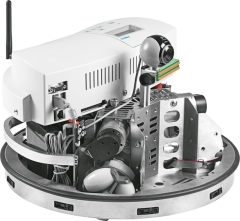
\includegraphics[width=0.8\textwidth]{img/robotino/d750242uc.jpg}
\caption[Robotiono]{Robotino des Unternehmens Festo Didactic, Quelle: Festo Didactic\footnotemark[13]}
\label{fig:robotino}
\end{figure}

\footnotetext[13]{\href{http://www.festo-didactic.com/de-de/lernsysteme/robotino-forschen-und-lernen-mit-robotern/szenarien-und-lernfelder.htm?fbid=ZGUuZGUuNTQ0LjEzLjE4Ljg1OC40NzU1}{\enquote{Robotino\textsuperscript{\textregistered} – Szenarien und Lernfelder}}. festo-didactic.com. Abgerufen Mai 26, 2013}
\newpage
\clearpage

\subsection{Lego Mindstorms NXT}

Vom Spielwarenhersteller LEGO werden unter dem Namen Mindstorms\footnotemark[14] Sets zur Entwicklung verschiedener Roboter vertrieben. Kern des Sets ist der sogennante NXT-Brick, ein intelligenter Baustein zur Ansteuerung der verschiedenen Sensoren und Aktoren, die ebenfalls zum Set geh\"oren. Der NXT wird seit 2006 vertrieben, wird jedoch noch dieses Jahr durch einen aktuelleren Baustein, den EV3\footnotemark[15] abgel\"oest werden.

\footnotetext[14]{\href{http://http://mindstorms.lego.com/en-us/default.aspx}{Website der LEGO Mindstorms}. mindstorms.lego.com. Abgerufen Mai 26, 2013}
\footnotetext[15]{\href{http://mindstorms.lego.com/en-us/News/ReadMore/Default.aspx?id=476243}{Announcing LEGO MINDSTORMS EV3}. mindstorms.lego.com. Abgerufen Mai 26, 2013}

Die Hardware des Lego Mindstorms NXT in der Version 2.0 ist wie folgt spezifiziert\footnotemark[16]: 

\footnotetext[16]{\href{http://de.wikipedia.org/wiki/NXT}{NXT - Hardware-Spezifikation des NXT-Steins}. de.wikipedia.org. Abgerufen Mai 26, 2013}

\begin{itemize}
\item Atmel-ARM-Prozessor, AT91SAM7S256; 256 kB Flash-Speicher, 64 KB RAM, 48 MHz
\item Koprozessor: Atmel 8-Bit AVR, ATmega48; 4 KB Flash-Speicher, 512 Byte RAM, 8 MHz
\item Bluetooth: CSR BlueCore 4 v2.0 +EDR; unterstützt das Serial Port Profile (SPP), 26 MHz
\item USB-2.0-Anschluss, 12 Mbit/s
\item 3 Motorausgänge mit Rückkanal
\item 4 Sensoreingänge, analog und digital kombiniert
der vierte Eingang kann als High-Speed-Port, entsprechend IEC 61158 Type 4/EN 50170, genutzt werden
\item Punktmatrix LC-Anzeige; 100 x 64 Pixel, Abmessungen: 26 x 40,6 mm
\item Soundausgabe mit 8-Bit-Auflösung und einer Samplingrate von 2 bis 16 kHz
\item Open Source Firmware
\end{itemize}


Sensoren für den Lego Roboter werden von der Firma HiTechnic entwickelt.
In den folgenden Kategorien sind Sensoren verf\"ugbar:

\begin{itemize}
\item Infrarot-Sucher
\item Kreisel-Sensor
\item Farbsensor
\item Beschleunigungssensor
\item Kompass-Sensor
\item Temperatur-Sensor
\item EOPD-Sensor
\end{itemize}

Trotz dessen, dass es sich bei diesem Modell um ein Spielzeug handelt, ist es aufgrund der vielen verf\"ugbaren Sensoren, sowie der Unterst\"utzung der Entwicklung durch Ver\"offentlichung der Hardware Spezifikationen, wie auch Developer-Toolkits, eine attraktive Platform zur Anwendung im Bereich der Robotik.  

\begin{figure}[H]
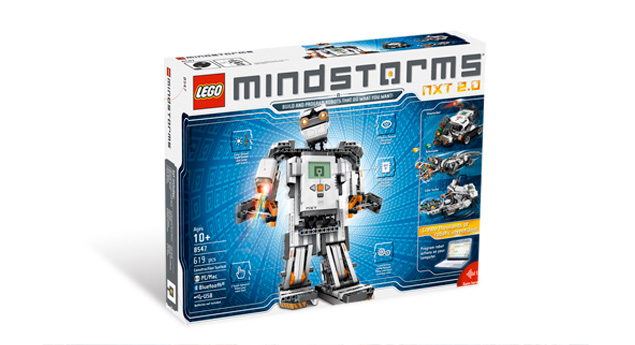
\includegraphics[width=0.8\textwidth]{img/nxt/download8BECFDA0517A505735D8E38A0137B963.jpg}
\caption[LEGO Mindstorms Set NXT 2.0]{LEGO Mindstorms Set NXT 2.0, Quelle: Festo Didactic\footnotemark[17]}
\label{fig:nxt_fig}
\end{figure}

\footnotetext[17]{\href{http://mindstorms.lego.com/en-us/products/default.aspx}{Produktsteite des NXT}. mindstorms.lego.com. Abgerufen Mai 26, 2013}
\clearpage

\subsection{Sphero}

Der Sphero\footnotemark[18] des Unternehmens Orbotix ist eine Roboterkugel. Er kann mittels Bluetooth angesteuert werden und verf\"ugt auch \"uber Sensoren, ein Gyroskop, ein Beschleunigungssensor und ein Kompass\footnotemark[19]. Die Entwicklung von Anwendungen f\"ur den Sphero wird vor allem auf den mobilen Platformen Android und iOS unterst\"utzt, es existieren jedoch auch inoffizielle Framewrosk zur Verwendung des Roboters in anderen Programmiersprachen und -umgebungen.

\footnotetext[18]{\href{http://www.gosphero.com/sphero/overview/}{Produkts\"ubersicht des Sphero}. gosphero.com. Abgerufen Mai 26, 2013}
\footnotetext[19]{\href{http://www.heise.de/hardware-hacks/meldung/Angerollt-Roboter-Kugel-Sphero-1542563.html}{Angerollt: Roboter Kugel Sphero}. heise.de. Abgerufen Mai 26, 2013}

\begin{figure}[H]
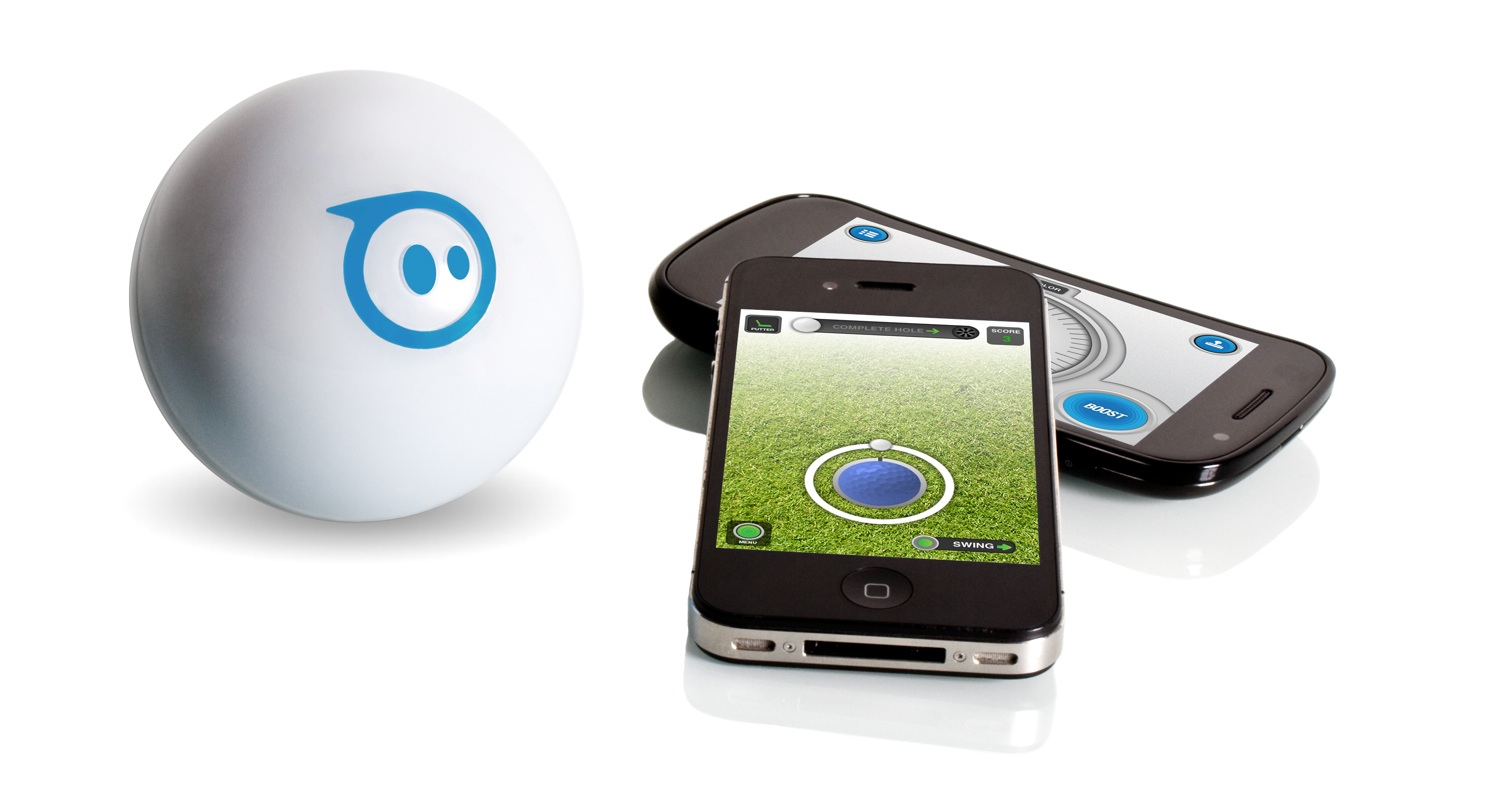
\includegraphics[width=0.8\textwidth]{img/sphero/Sphero1.jpg}
\caption[Roboter Kugel Sphero]{Roboter Kugel Sphero, Quelle: Wired\footnotemark[20]}
\label{fig:sphero}
\end{figure}

\footnotetext[20]{\href{http://www.wired.com/reviews/2011/12/sphero/}{Orbotix Sphero - The Shape of Things to Come}. wired.com. Abgerufen Mai 26, 2013}

\clearpage

Wie auch beim LEGO Roboter NXT handelt es sich hierbei im Grunde um ein Spielzeug. Doch auch hier gibt es Portierungen des SDK die die anderweitige Verwendung der Kugel erm\"oglichen. Auch dieser Roboter erf\"ullt grunds\"atzlich, die durch das Projekt vorgegebenen Anforderungen. 

\section{Umsetzung mit dem LEGO Mindstorms NXT}

Im Rahmen dieses Projektes wird der NXT 2.0 aus der Lego Mindstorm Serie eingesetzt\footnotemark[21]. Im Kontext dieser Arbeit sind keine Sensoren notwendig, da der Roboter aus der Ferne gesteuert wird. Die grunds\"atzlichen Anforderungen werden von allen vorgestellten Robotermodellen unterst\"utzt. Der Lego Mindstorms NXT wurde in erster Linie ausgew\"ahlt, da die Duale Hochschule hier \"uber viele Modelle verf\"ugt. Somit war es m\"oglich den Roboter auszuleihen und wesentlich flexibler mit der Entwicklung der Schnittstelle umzugehen, als dies mit den anderen Modellen m\"oglich gewesen w\"are. Ebenfalls ausschlaggebend war die die Unterst\"utzung durch Frameworks zur Entwicklung, welches im Falle des NXT durch das Framework leJOS optimal gegeben war. Mehr hierzu im nachfolgenden Kapitel \ref{chap:Lego-Framework}.

\footnotetext[21]{\href{http://mindstorms.lego.com/en-us/products/default.aspx}{\enquote{LEGO® MINDSTORMS® NXT 2.0}}. mindstorms.lego.com. Abgerufen Mai 24, 2013}

\par\smallskip    
Der eingesetzte Roboter ist in der nachfolgenden Abbildung \ref{fig:nxt} dargestellt. Das Modell ist so aufgebaut, dass mittels eines Motors der Antrieb, mit der anderen die Lenkung mit einer Lenkachse realisiert ist.

\begin{figure}[H]
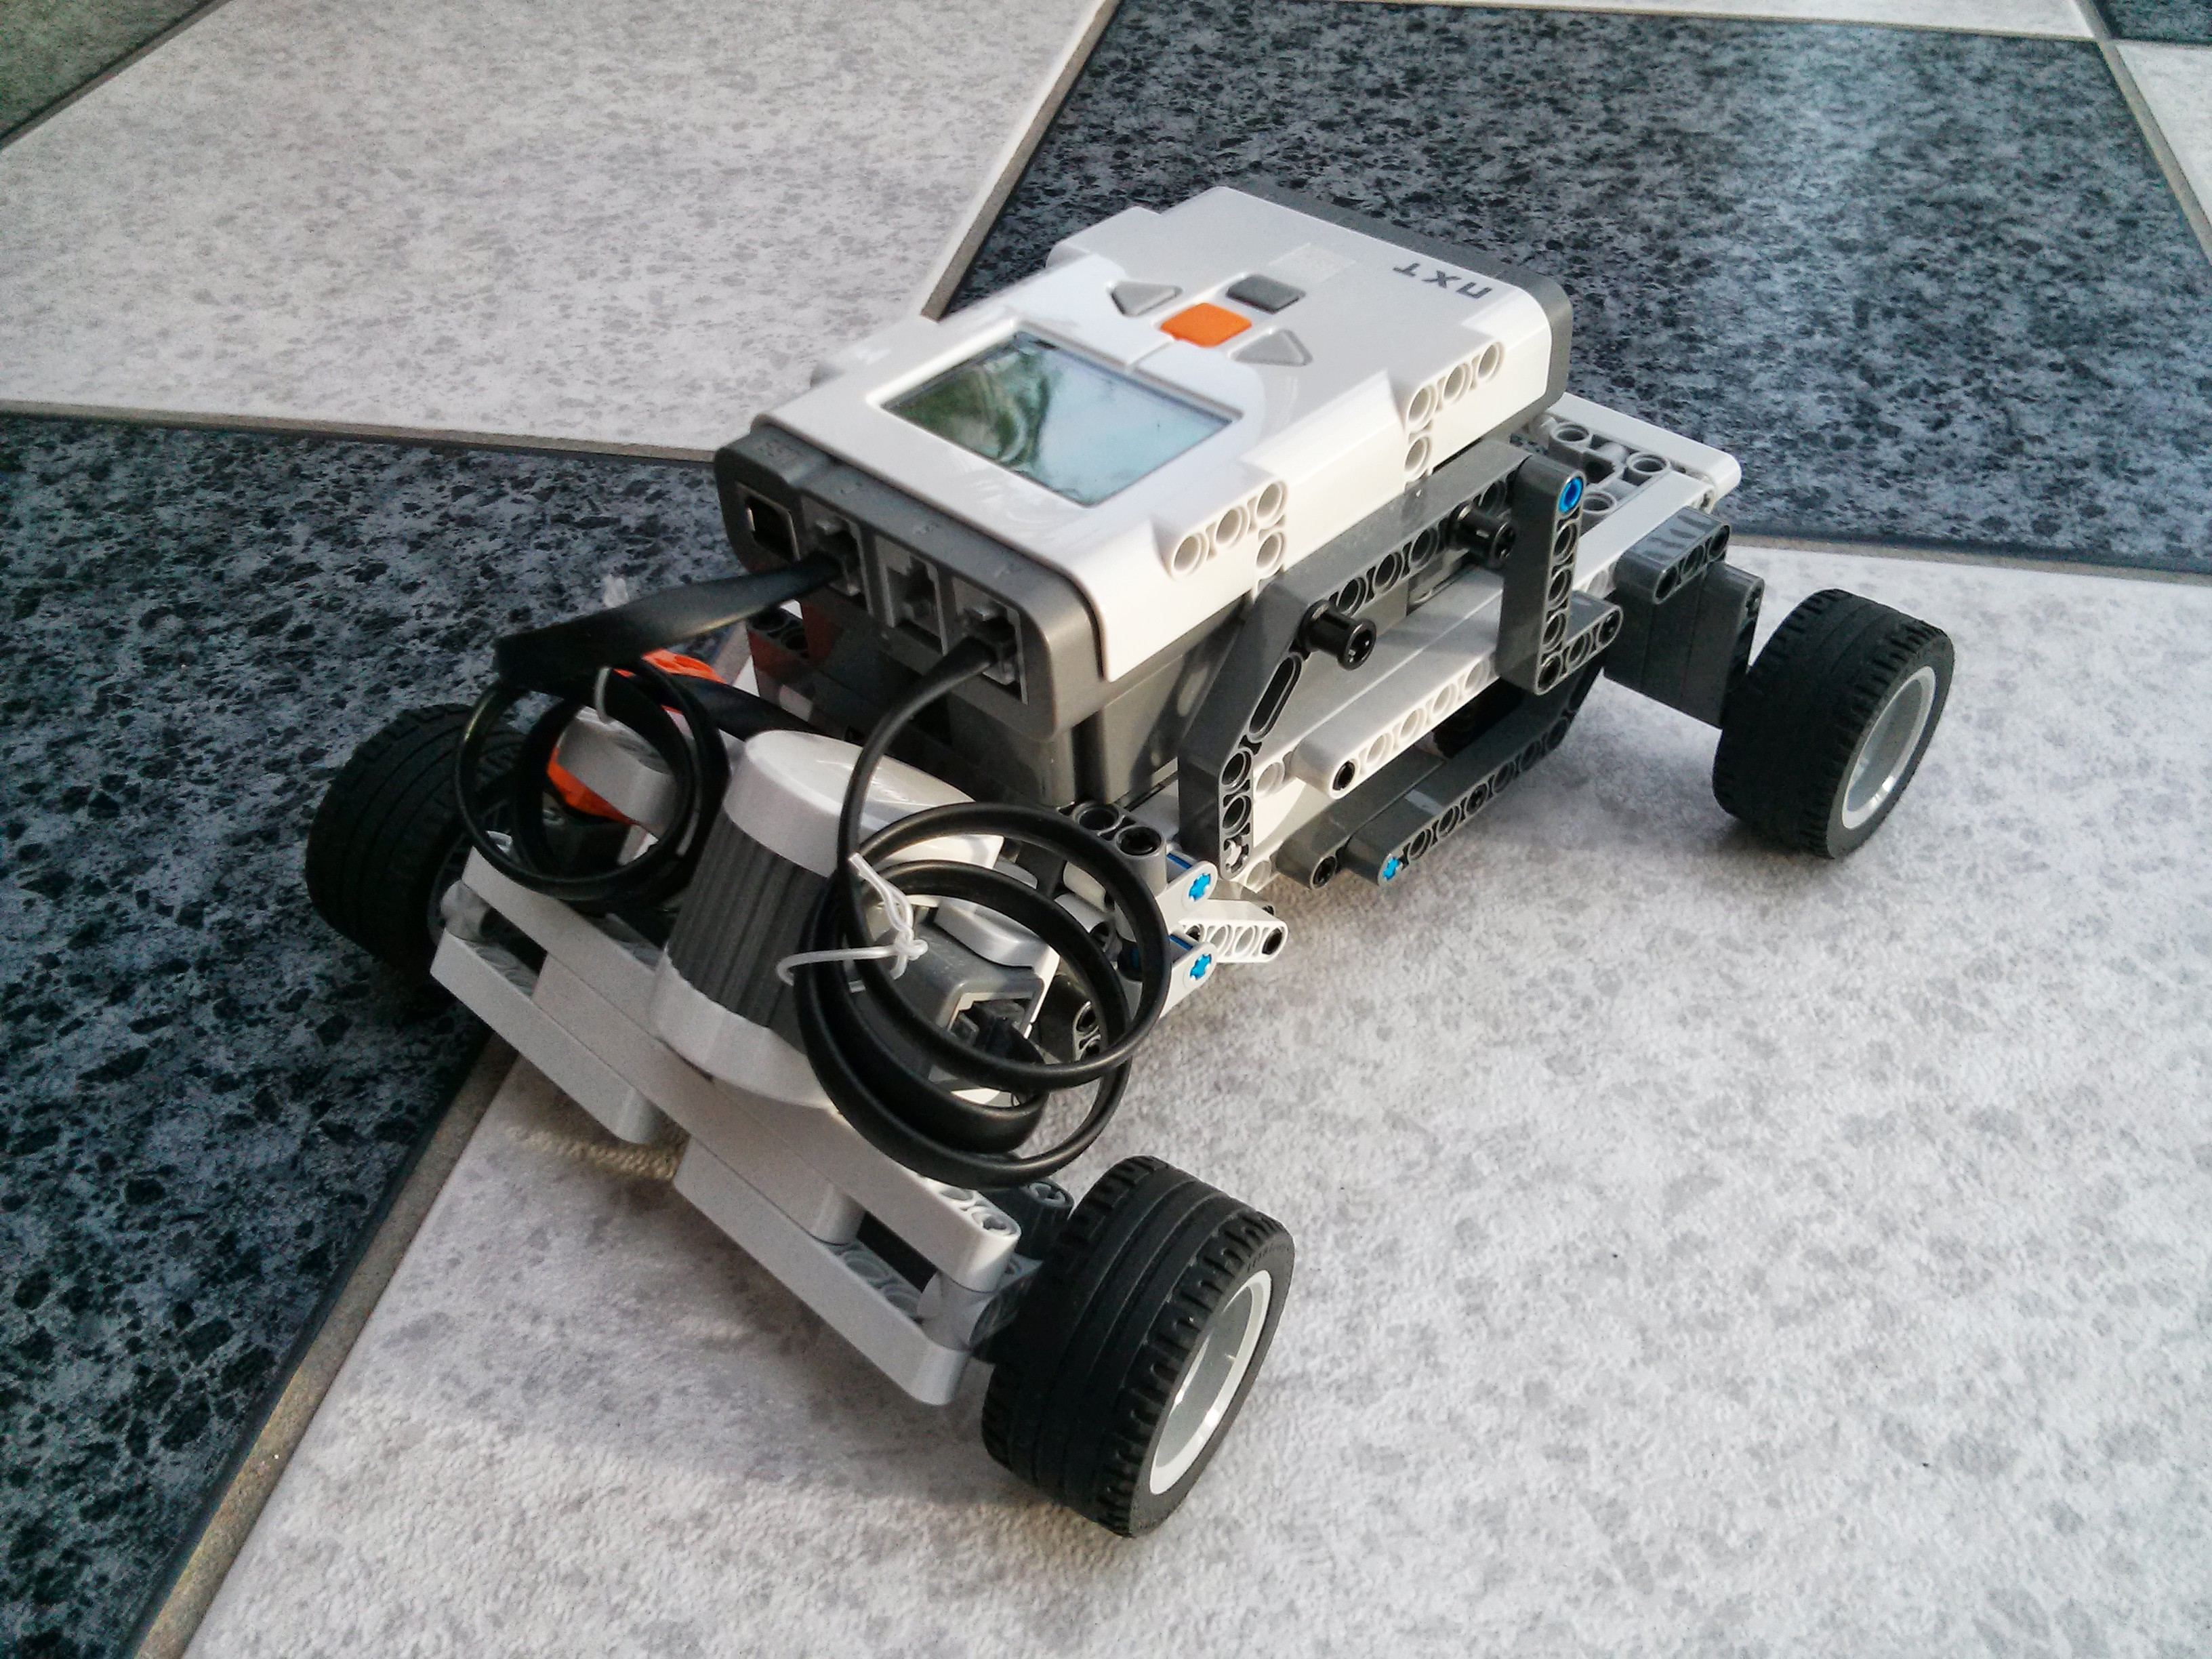
\includegraphics[width=0.8\textwidth]{img/nxt/IMG_20130603_065536.jpg}
\caption[NXT]{NXT Robotermodell mit Lenkachse}
\label{fig:nxt}
\end{figure}
\clearpage